\documentclass[letter,openrigh,12pt,spanish]{report}
%Gummi|065|=)
\title{\textbf{Describir las caracter\'isticas de cinem\'atica directa e inversa de manipuladores paralelos.}}
\author{Diego Armando Becerra Iñiguez\\
		Cineamtica de Robots\\
		Ing. Mecatr\'onica 7to A}
\date{28 de febrero de 2019}
\usepackage{amsmath}
\usepackage{graphicx}
\begin{document}

\maketitle

\section{Cinematica Directa.}

Utilizando la notaci\'on de Denavit y Hartenberg se puede expresar la posici\'on y orientaci\'on del efector final del manipulador en funci\'on del desplazamiento de sus articulaciones. El desplazamiento articular es un \'angulo ($\theta_i$) o una distancia ($d_i$), dependiendo del tipo de articulaci\'on.

Los robots paralelos donde el n\'umero de cadenas es estrictamente igual al n\'umero de GDL del efector final son llamados manipuladores paralelos completos. Hay dos casos de robots paralelos: planos, esfericos o espaciales. Un robot completamente paralelo plano tiene 3 GDL en su efector final, dos de traslaci\'on y uno de rotaci\'on. Un robot completamnete paralelo con \textit{m} GDL posee \textit{m} cadenas unidas a su efector final. SI las cadenas son identicas se puede utilizar la formula de Gruber's, aunque algunas veces esta f\'ormula puede tener errores debido a que no considera las relaciones geometricas entre las juntas.

Un manipulador paralelos se puede considerar como sim\'ertrico si se satisfacen las siguientes condiciones:

1. el n\'umero de cadenas es igual al n\'umero de grados de libertad de la plataforma m\'ovil.

2.EL tipo y n\'umero de juntos de todas las cadenas son iguales.

3. El n\'umero y la localizaci\'on de las juntas activas en todas las cadenas son las mismas.

\subsection{Robots paralelos planos}

Para definir un cuerpo plano cartesiano se necesitan dos coordenadas y un \'angulo, en el caso de los manipuladores paralelos planos de 2 grados de libertad s\'olo se pueden describir por dos coordenadas ya sean cartesianas o polares y en el caso de manipuladores paralelos planos de 3 grados de libertad se pueden describir las dos coordenadas y la orientaci\'on.

\subsubsection{Robots paralelos planos de 2 GDL}

Los robots paralelos planos de 2 grados de libertad est\'an formados por paralelogramos que permiten que el eslab\'on de salida permanezcan en una orientaci\'on fija con respecto al eslab\'on de entrada, las ventajas son la capacidad de rotaci\'on altas. JX Liu, en 2003, presenta mecanismos paralelos que tienen amplias aplicaciones en robots industriales, simuladores, micromanipuladores, maquina denominadas de cinem\'atica paralela, y cualquier otro dispositivo de manipualci\'on en los que se necesitan alta capacidad de rotaci\'on y alta rigidez. Sobre todo, presenta nuevos conceptos de dise\~no de mecanismos paralelos, novedosos y la mejora de la capacidad de rotaci\'on de dichos sistemas.

En la \ref{Figure 1} se muestran algunas arquitecturas de manipuladores paralelos de 2 GDL. Presentados por Figielski, 2007, los cuales est\'an formados por juntas rotaciones y juntas prism\'aticas.

\begin{figure}[htp]
\centering
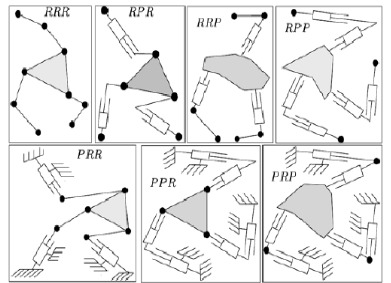
\includegraphics[scale=1.00]{1.jpg}
\caption{Robots paralelos de 2 GDL}
\label{Figure 1}
\end{figure}

\subsubsection{Robots paralelos de planos de 3 GDL}

En los manipuladores paraleos de 3 GDL, se asume que cada cadena cuenta con tres juntas y dos eslabones. Utilizando juntas rotacionales \textit{R} y juntas prismaticas \textit{P}. Cada una de las cadenas cinem\'aticas independientes se denota por un conjunto de tres letras que indican la sucesi\'on de las juntas a partir de la tierra. Las cobinaciones son, por tanto: \textit{RRR}, \textit{RPR}, \textit{PPR}, \textit{RRP}, \textit{PRP}, \textit{PPP}, la configuraci\'on \textit{PPP} presenta movimientos independientes. Si se asume que las tres cadenas cinem\'aticas son id\'enticas, se presentan todas las configuraciones posibles en la \ref{Figure 2}

\begin{figure}[htp]
\centering
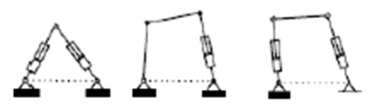
\includegraphics[width=8cm]{2.jpg}
\caption{Manipuladores paralelos planos de 3GDL}
\label{Figure 2}
\end{figure}

El plano paralelo plano est\'a constituido por una plataforma m\'ovil, conectada a tierra por tres cadenas cinematicas independientes que tienen tres grados de libertad, independientes una aticulaci\'on es accionada.

Las cadenas cinem\'aticas de cualquier manipulador plano completo pueden estar compuestas en cada cadena por cualquier secuencia de las juntas que se muestran en la \ref{Tabla 1}

\begin{center}
\begin{table}
\begin{tabular}{|c|c|c|c|c|c|}
\hline
	RRR & RRR & RRR & RPR &  RPR & RPR\\
\hline
	RPP & RPP & PRR & PRR & PRR & PRP\\
\hline
	PRP & PPR & PPR & RRP & RRP & RRP\\
\hline
\end{tabular}
\caption{Cadenas cinem\'aticas robot 3GDL}
\label{Tabla 1}
\end{table}
\end{center}

Los manipuladores paralelos planos se definen por la secuencia que describe las tres cadenas cinem\'aticas, por ejemplo Gosselin y Angeles en 1988, presentan el robot paralelos 3RRR que es el robot con tres cadenas cinem\'aticas RRR. Entre los investigadores que realizaron un extenso estudio sobre estos robots, se encuentran Kassner, Gosselin. Por otro lado la s\'intesis dimensional ha sido abordad por Shikbodaie, 1987 y Arsenault, 2004, an\'alisis de singularidades por Gosselin y espacio de trabajo Kumar, 1992. Lui, 200, Gao 2001, rigidez Kim, 2000.

\section{Cinematica inversa}

Para los manipuladores paralelos la cinem\'atica inversa resulta ser m\'as simple, en compraci\'on con la cinematica directa.

En robots paralelos la cinem\'atica inversa consiste en establecer el valor de las juntas activas y pasivas en funci\'on de las coordenadas del extremo del robot, las juntas activas son las juntas actuadas y las juntas pasivas son las que quedan en funci\'on de las juntas activas. Establecer la cinem\'atica inversa es esencial para el control de la posici\'on de los robots paralelos. EL mapeo de la cinem\'atica, tiene interesantes ecuaciones algebraicas que tienen m\'ultiples soluciones. La cinem\'atica inversa de los manipuladores paralelos en general es id\'entica a la de los manipuladores serie.

En la cinem\'atica directa de robots paralelos el problema es determinar la posici\'on del efector final en funci\'on de las juntas activas. En general, las soluciones para este problema no es \'unico, es decir, hay varias maneras de atacar a un manipulador paralelo. En el estudio de la cinem\'atica directa Merelt, Tsai, Angeles, Raghavan, recurrieron a la soluci\'on de un polinomio mostraron que el problema de la cinam\'atica directa es reducir la soluci\'on a polinomio.

Es importante hacer incapie en el problema de la validacion de resultado de la cinem\'atica directa por polinomios, el c\'alculo puede implicar un gran n\'umero de operaciones y por lo tanto puede ser muy sencible a errores numericos de redondeo, por lo que la comprobaci\'on de la validez de las soluciones con la cinem\'atica inversa puede ser necesario.

\begin{thebibliography}{X}
\bibitem{Robot} \textbf{Patricio Martinez Zamudio.} (2015). Manipulador paralelo 3RRR . Mexico, D.F: UNAM.
\end{thebibliography}

\end{document}
